\documentclass{standalone}
\usepackage{tikz}
\usepackage{pgfplots}
\pgfplotsset{compat=1.18}
\usetikzlibrary{calc, decorations.markings, arrows.meta}

\begin{document}
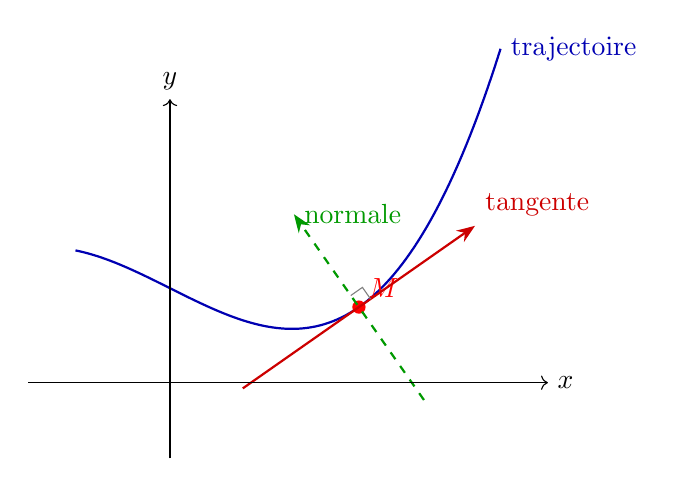
\begin{tikzpicture}[scale=1.2]

  % --- Paramètres du point d'intérêt ---
  % Trajectoire : y = f(x) = 0.1*x^3 - 0.5*x + 1
  % Dérivée     : f'(x)   = 0.3*x^2 - 0.5
  % On choisit  : x0 = 2

  \pgfmathsetmacro{\xzero}{2}
  \pgfmathsetmacro{\yzero}{0.1*\xzero^3 - 0.5*\xzero + 1}       % f(x0)
  \pgfmathsetmacro{\slope}{0.3*\xzero^2 - 0.5}                    % f'(x0)
  \pgfmathsetmacro{\normalslope}{-1/\slope}                        % pente normale = -1/f'(x0)
  \pgfmathsetmacro{\tanglen}{1.5}   % demi-longueur tangente affichée
  \pgfmathsetmacro{\normlen}{1.2}   % demi-longueur normale affichée

  % Vecteur directeur unitaire de la tangente
  \pgfmathsetmacro{\tx}{1/sqrt(1+\slope*\slope)}
  \pgfmathsetmacro{\ty}{\slope/sqrt(1+\slope*\slope)}

  % Vecteur directeur unitaire de la normale (rotation 90°)
  \pgfmathsetmacro{\nx}{-\ty}
  \pgfmathsetmacro{\ny}{\tx}

  % --- Trajectoire ---
  \draw[thick, blue!70!black, samples=100, domain=-1:3.5,
        /pgf/declare function={f(\x) = 0.1*\x^3 - 0.5*\x + 1;}]
    plot (\x, {f(\x)}) node[right] {trajectoire};

  % --- Point M sur la trajectoire ---
  \fill[red] (\xzero, \yzero) circle (2pt) node[above right] {$M$};

  % --- Tangente en M ---
  \draw[red!80!black, thick, -Stealth]
    ({\xzero - \tanglen*\tx}, {\yzero - \tanglen*\ty})
    -- ({\xzero + \tanglen*\tx}, {\yzero + \tanglen*\ty})
    node[above right] {tangente};

  % --- Normale (perpendiculaire à la tangente) en M ---
  \draw[green!60!black, thick, dashed, -Stealth]
    ({\xzero - \normlen*\nx}, {\yzero - \normlen*\ny})
    -- ({\xzero + \normlen*\nx}, {\yzero + \normlen*\ny})
    node[right] {normale};

  % --- Angle droit (marqueur visuel) ---
  \pgfmathsetmacro{\sqsize}{0.15}
  \draw[gray]
    ({\xzero + \sqsize*\tx}, {\yzero + \sqsize*\ty})
    -- ({\xzero + \sqsize*\tx + \sqsize*\nx}, {\yzero + \sqsize*\ty + \sqsize*\ny})
    -- ({\xzero + \sqsize*\nx}, {\yzero + \sqsize*\ny});

  % --- Axes ---
  \draw[->] (-1.5,0) -- (4,0) node[right] {$x$};
  \draw[->] (0,-0.8) -- (0,3)  node[above] {$y$};

\end{tikzpicture}
\end{document}